\newgeometry{textwidth=16cm}
\chapter[Rappels théoriques : DFT]{Rappels théoriques : Méthodes de la fonctionnelle de la densité (DFT)}
\minitoc
\restoregeometry

\newpage

\section*{Introduction}
\markright{INTRODUCTION}{}

La chimie théorique est une science relativement récente, puisque ce n'est qu'en 1933 que le physicien autrichien Erwin Schr\"{o}dinger  a reçu le prix \textsc{Nobel} de physique, en commun avec Paul \textsc{Dirac}, pour ses travaux représentant, depuis, les fondements de la chimie quantique. En effet, l'équation de Schr\"{o}dinger nous prouve que la connaissance de la fonction d'onde du système donne accès, explicitement ou non, à toutes les valeurs caractéristiques du système chimique étudié. Dans l'article \textit{La situation actuelle en mécanique quantique}~\cite{schrodinger1992situation} paru en 1935, la métaphore du  \og chat de Schr\"{o}dinger \fg{} a largement contribué à la vulgarisation de cette science auprès du public scientifique. En effet, il y symbolise, à l'aide d'un exemple macroscopique régit par les lois de la physique classique, la philosophie de la mécanique quantique dévolue à l'étude des systèmes microscopiques. Le plus grand défi à relever ici était de faire comprendre qu'une \og mesure quantique \fg{} est une combinaison linéaire d'une somme d'états de probabilités non-nulles et non une valeur unique. L'expérience fictive consiste à placer un chat dans une boîte contenant un flacon de poison ainsi qu'une source radioactive. Lorsqu'un compteur Geiger détecte un certain seuil de radiation, un mécanisme vient briser le flacon et libère ainsi des vapeurs mortelles. Dans un raisonnement quantique, le chat est donc à la fois vivant \underline{et} mort dans la boîte tant qu'elle reste close, avec une probabilité de vie de plus en plus faible au cours du temps.\\

En pratique, le nombre considérable de calculs à réaliser dans le cadre de la chimie théorique lie intrinsèquement cette science au développement de l'informatique, tout aussi récent. Il s'agit même de l'une des plus grandes limites encore rencontrée de nos jours. Même si la loi de \textsc{Moore}~\cite{moore1965electronics}~\footnote{La loi de \textsc{Moore} (1965), renommée première loi de \textsc{Moore} compte-tenu de l'ajustement ultérieur, énonce que la complexité des semi-conducteurs (et donc de la puissance de calcul) suit une loi exponentielle au cours du temps.}, empirique de son état, a commencé à perdre en véracité dès lors que la fréquence des processeurs (CPU) engendrait une déperdition de chaleur trop importante et commercialement non-maîtrisable ($\gtrsim$ 5 Ghz), l'apparition des processeurs multic\oe urs s'est vu être la solution la plus efficace. Après l'adaptation nécessaire des codes séquentiels en version parallèle, la démocratisation relative des clusters de calcul~\footnote{Un cluster de calcul, ou grappe de serveurs, est un ensemble de serveurs esclaves, les n\oe uds, contrôlés par un ou plusieurs serveurs maîtres, le(s) frontal(aux). Ce groupe de serveurs indépendants, fonctionnant comme un seul et même système, permet d'optimiser les ressources (processeur, mémoire vive, stockage\dots{}) et une meilleure répartition des tâches sur les différents n\oe uds.} permet à l'heure actuel le développement de codes hautement parallélisés (> 1000 processeurs). Ceci permet alors de faire moins d'approximations théoriques et donc de tendre vers des valeurs de plus en plus exactes, tout en gardant des temps de calcul raisonnables. Un engouement pour les clusters de cartes graphiques (GPU) est aussi à noter dans les domaines scientifiques où, tel que la dynamique moléculaire, les calculs sont extrêment fragmentables et peu interdépendants.\\

Dans ce chapitre, nous rappellerons dans un premier temps les fondements de la théorie de la fonctionnelle de la densité, notée DFT, par le biais de l'évolution des différents modèles qui ont été proposés. Nous verrons ensuite comment les théorèmes de \textsc{Hohenberg} et \textsc{Kohn} prouvent que la seule connaissance de la densité électronique permet de résoudre l'équation de Schr\"{o}dinger dans le cadre de la DFT. La fonctionnelle universelle $F_{HK}[\rho]$, qui permettrait une résolution exacte du problème, restant inconnue, nous aborderons dans une troisième partie l'approche KS qui contourne ce problème et légitime certaines approximations. Ces dernières donnant naissance à différents types de fonctionnelle, elles seront succintement présentées dans la pénultième partie de ce chapitre. Finalement, le développement de la méthode de calcul utilisée dans ce travail de thèse, sera présentée étape par étape en fin de chapitre. 

\newpage

\section{Les fondements de la DFT}

Contrairement aux méthodes HARTREE-FOCK, noté HF, et \textit{a fortiori} post-HF qui décrivent le système électronique par une fonction d'onde $\Psi_{(\vec{r})}$, la théorie de la fonctionnelle de la densité le décrit par la densité électronique, notée $\rho_{(\vec{r})}$, qui est liée à la fonction d'onde $\Psi_{(\vec{r})}$ par la relation suivante~:

\begin{align}
\rho_{(\vec{r})} &= \int \Psi_{(\vec{r})}^{*} \Psi_{(\vec{r})} \\
&= \int |\Psi_{(\vec{r})}^{2}| \notag
\end{align}

\begin{flushleft}
\begin{tabular}{@{}lrp{10cm}}
avec & $\vec{r}$ : & ensemble des coordonnées électroniques. 
\end{tabular}
\end{flushleft}


L'énergie de l'état fondamental est ainsi une fonctionnelle de la densité électronique, c'est-à-dire que $E_{0} = E_{(\rho)}$.

\subsection{Modèle de \textsc{Thomas-Fermi}}

Le terme d'énergie cinétique a été exprimé comme une fonctionnelle de la densité pour la première fois en 1927 par \textsc{Thomas} et \textsc{Fermi}~:

\begin{equation}
\hat{T}_{TF}[\rho] = \frac{3}{10} (3\pi)^{2/3} \int \rho_{(\vec{r})}^{5/3} .d\vec{r}
\label{ener_cin_thom_ferm}
\end{equation}

Celle fonctionnelle est alors combinée aux expressions classiques des interactions électrons-noyaux et électrons-électrons, exprimées elles aussi en fonction de la densité électronique :

\begin{equation}
E_{TH}[\rho] = T_{TH}[\rho] + V_{Ne}[\rho] + V_{ee}[\rho]
\end{equation}

\subsection{Modèle de \textsc{Thomas-Fermi-Dirac}}

Le terme d'échange, résultant du principe d'exclusion de \textsc{Pauli}, a ensuite été ajouté par Dirac en 1930 afin d'affiner le modèle :

\begin{align}
K[\rho] = E_{x}[\rho] &= \int \rho_{\vec{r}} \epsilon_{x}[\rho] .d\vec{r} \\
&= -\frac{3}{4} \left(\frac{3}{\pi}\right)^{1/3} \int \rho_{(\vec{r})}^{4/3} .d\vec{r} \notag
\end{align}

\begin{flushleft}
\begin{tabular}{@{}lrp{10cm}}
avec & $\epsilon_{X}[\rho]$ : & énergie d'échange par électron. 
\end{tabular}
\end{flushleft}

Le modèle de \textsc{Thomas-Fermi-Dirac} est défini par la combinaison de cette expression avec l'équation~\ref{ener_cin_thom_ferm} et le potentiel d'interaction électrons-noyaux $V_{Ne}[\rho]$. Notons que la corrélation électronique n'est toujours pas prise en compte dans ce modèle.

\subsection{Modèle de \textsc{Slater}}

Partant d'une approche basée sur la méthode HF, \textsc{Slater} proposa en 1951 de substituer le terme d'énergie d'échange par une fonctionnelle de la densité issue de l'énergie d'échange de Dirac. Ce terme d'échange dans le formalisme HF peut alors être généralisé en introduisant le paramètre $\alpha$ :

\begin{equation}
E_{x}[\rho] = - \frac{9\alpha}{8} \left(\frac{3}{\pi}\right)^{1/3} \int \rho_{(\vec{r})}^{4/3} .d\vec{r}
\end{equation}

Des analyses empiriques basées sur différents types de systèmes chimiques ont conduit à une valeur de $3/4$ pour $\alpha$, offrant une meilleure précision que la valeur originelle de l'expression de Dirac ($2/3$).

\section{Les théorèmes de \textsc{Hohenberg} et \textsc{Kohn}}

Tous ces modèles, qui constituent les fondements de la DFT, ne démontrent pas formellement que seul la connaisance de la densité est importante pour atteindre la valeur de l'énergie totale d'un système. C'est ainsi que \textsc{Hohenberg} et \textsc{Kohn} eurent l'idée en 1965 de démontrer, par le biais de deux théorèmes, que l'équation de Schr\"{o}dinger pouvait être résolue de façon exacte, dans le cadre de l'approximation de \textsc{Born-Oppenheimer} uniquement grâce à la densité électronique.

\subsection{Premier théorème : preuve d'existence}

Ce premier théorème énonce que l'ensemble des propriétés du système, notamment l'énérgie, peuvent être calculées à partir de la seule densité électronique de l'état fondamental. Elles peuvent donc être décrites comme une fonctionnelle de la densité électronique, et l'énergie totale s'écrit alors :

\begin{equation}
E[\rho] = F_{HK}[\rho] + \int \rho_{(\vec{r})} \nu_{ext} .d\vec{r}
\label{Hohen_Kohn}
\end{equation}
\noindent où :
\begin{align}
F_{HK}[\rho] &= T_{e}[\rho] + V_{ee}[\rho] \\
\nu_{ext} &= V_{Ne}[\rho] \notag
\end{align}

Notons que la fonctionnelle universelle $F_{HK}[\rho]$, qui regroupe les termes d'énergie cinétique des électrons et celui d'énergie potentielle d'interaction électron-électron, n'est pas liée au potentiel externe $\nu_{ext}$. L'énergie de l'état fondamental est \textit{a priori} accessible de manière exacte car cette fonctionnelle ne repose sur aucune approximation.

\subsection{Second théorème : théorème variationnel}

Basé sur l'équation~\ref{Hohen_Kohn}, \textsc{Hohenberg} et \textsc{Kohn} ont ensuite construit un principe variationnel pour déterminer la densité électronique de l'état fondamental :

\begin{equation}
E[\rho] \geq E[\rho_{0}]
\end{equation}

\begin{flushleft}
\begin{tabular}{@{}lrp{10cm}}
avec & $\rho_{0}$ : & densité électronique de l'état fondamental, \\
& $\rho$ : & densité électronique quelconque.
\end{tabular}
\end{flushleft}

Dans cette équation, à une densité d'essai $\rho$ correspond une seule énergie potentielle $\int \rho_{(\vec{r})} \nu_{ext} .d\vec{r}$ et une seule fonction d'onde $\Psi_{\rho}$. La méthode de double minimisation, \textit{i.e.} sous contrainte de \textsc{Levy}, permet de différencier la fonction d'onde $\Psi_{\rho_{0}}$, correspondant à l'état fondamental, parmi le jeu infini des fonctions d'ondes $\Psi_{\rho}$ donnant la même densité. Ainsi, nous pouvons déterminer, parmi toutes les densités, celle qui minimisera l'énergie par la relation suivante :

\begin{equation}
E[\rho_{0}] = \min\limits_{\rho}\, (\min\limits_{\Psi\rightarrow\rho}\, (F[\rho] + \int \rho_{\vec{r}} \nu_{\vec{r}}\, .d\vec{r}\, ))
\end{equation}

Si les théorèmes de \textsc{Hohenberg} et \textsc{Kohn} démontrent une correspondance unique entre une densité $\rho_{\vec{r}}$ et la fonction d'onde $\Psi$ du système, la fonctionnelle universelle $F_{HK}[\rho]$ reste cependant inconnue.

\section{Approche Kohn-Sham}\label{Kohn-Sham}

Afin de contourner ce problème, \textsc{Kohn} et \textsc{Sham} substituèrent au Hamiltonien réel, décrivant un système de $n$ particules en interaction, un Hamiltonien de référence décrivant un système de $n$ particules sans interaction mais ayant la même densité que le système réel. Le problème est ainsi réduit à la résolution de $n$ équations monoélectronique couplées, analogues aux équations de HF. L'opérateur monoélectronique de Kohn-Sham $\hat{K}_{KS}$ s'exprime ainsi :

\begin{equation}
\hat{H}_{KS} = -\frac{1}{2} \nabla^{2} + \nu_{H}[\rho] + \nu_{xc}[\rho] + \nu_{ext}[\rho]
\end{equation}

\noindent où :
\begin{align}
\nu_{H}[\rho] &= \int \frac{\rho_{(\vec{r})} - \rho_{(\vec{r}')}}{|\vec{r} - \vec{r}'|} .d\vec{r}' \\
\nu_{xc}[\rho] &= \frac{\partial E_{xc}[\rho_{(\vec{r})}]}{\partial\rho_{(\vec{r})}}
\end{align}

\noindent $\nu_{H}[\rho]$ et $\nu_{xc}[\rho]$ étant respectivement le potentiel de \textsc{Hartree} et le potentiel d'échange et de corrélation, dans lequel $E_{xc}[\rho_{(\vec{r})}]$ est l'énergie d'échange et de corrélation.

En définissant un potentiel fictif $\nu_{eff(\vec{r})}$ pouvant être appliqué à des systèmes sans interaction de densité $\rho$ :

\begin{equation}
\nu_{eff(\vec{r})} = \nu_{H}[\rho] + \nu_{xc}[\rho] + \nu_{ext}[\rho]
\end{equation}

\noindent nous introduisons alors un jeu d'orbitales $\psi_{(\vec{r})}$, appelées orbitales de \textsc{Kohn-Sham}, et nous obtenons un jeu d'équations aux valeurs propres :

\begin{equation}
\hat{H}_{KS} \psi_{i(\vec{r})} = \epsilon_{i} \psi_{i(\vec{r})}
\end{equation}

Comme dans le cas de la méthode HF, l'énergie du système peut être minimisée en résolvant ce jeu d'équations de façon auto-cohérente grâce à l'utilisation des orbitales de \textsc{Kohn-Sham}. L'énergie du système est alors donnée par :

\begin{equation}
E_{KS}^{tot}[\rho] = T_{s}[\rho] + J[\rho] + E_{xc}[\rho] + \int V_{ext(\vec{r})}\rho_{(\vec{r})} .d\vec{r}
\end{equation}

\begin{flushleft}
\begin{tabular}{@{}lrp{10cm}}
avec & $T_{s}[\rho]$ : & énergie cinétique des électrons sans interaction, \\
& $J[\rho]$ : & énergie d'interaction coulombienne entre les électrons, \\
& $E_{xc}[\rho]$ : & énergie d'échange et de corrélation, \\
& $\int V_{ext(\vec{r})}\rho_{(\vec{r})} .d\vec{r}$ : & énergie d'interaction avec le potentiel externe. 
\end{tabular}
\end{flushleft}

D'après les théorèmes de \textsc{Hohenberg} et \textsc{Kohn}, $E_{KS}^{tot}[\rho]$ doit être égale à l'énergie totale du système réel $E_{reel}^{tot}[\rho]$, qui peut être décrite comme suit :

\begin{equation}
E_{reel}^{tot}[\rho] = T[\rho] + V_{ee}[\rho] + \int V_{ext(\vec{r})}\rho_{(\vec{r})} .d\vec{r}
\end{equation}

Le terme d'échange corrélation peut ainsi être explicité comme étant la somme de la correction à l'énergie cinétique due à l'interaction entre électrons ($T[\rho] - T_{s}[\rho]$) et les corrections non classiques à la répulsion électron-électron ($V_{ee}[\rho] - J[\rho]$) :

\begin{equation}
E_{xc}[\rho] = T[\rho] - T_{s}[\rho] + V_{ee}[\rho] - J[\rho]
\end{equation}

La théorie de la fonctionnelle de la densité de \textsc{Kohn-Sham} a connu un grand succès parmi les méthodes de calcul appliquées aux grands systèmes dû à son ratio coût calculatoire/performance très intéressant. C'est pour cet avantage indéniable qu'elle sert de base à de nombreuses évolutions de la DFT.

\section{Les différentes classes de fonctionnelle}

Formellement, la DFT est donc une méthode exacte, dans la limite de la connaissance de la fonctionnelle universelle $F_{HK}[\rho]$ ou de sa fonctionnelle exacte d’échange et de corrélation $F_{xc}[\rho]$. Malheureusement, la forme exacte de l’énergie d’échange et de corrélation est inconnue, si bien qu’il est nécessaire de faire des approximations. Dans la pratique, l’énergie d’échange et de corrélation $E_{xc}[\rho]$ est calculée à l’aide de fonctionnelles d’échange et de corrélation, définies comme suit :

\begin{equation}
\int F_{xc}[\rho_{(\vec{r})}].d\vec{r} = E_{xc}[\rho_{(\vec{r})}]
\end{equation}

L’énergie d’échange et de corrélation est généralement séparée en deux termes distincts, l’un d’échange $E_{x}[\rho]$ et l’autre de corrélation $E_{c}[\rho]$ :

\begin{equation}
E_{xc}[\rho_{(\vec{r})}] = E_{x}[\rho_{(\vec{r})}] + E_{c}[\rho_{(\vec{r})}]
\end{equation}

Plusieurs fonctionnelles ont donc été développées pour traiter chacune de ces contributions, de façon simultanée ou indépendante. Nous allons ici donner un bref aperçu -- non exhaustif -- des différentes familles de fonctionnelles, en suivant le critère de classification donné par \textsc{Perdew} et couramment dit \og échelle de Jacob de \textsc{Perdew} \fg{}. Il a proposé de classer les fonctionnelles en fonction du degré d’information non local contenu dans leur forme analytique. Au premier échelon se trouvent les fonctionnelles qui dépendent uniquement de la densité électronique, dites fonctionnelles LDA (\og Local Density Approximation \fg{}). Viennent ensuite les fonctionnelles corrigées par gradient GGA (\og Generalized Gradient Approximation \fg{}) dans lesquelles la non-localité est introduite grâce à leur dépendance par rapport au gradient de la densité. A ce même niveau se trouvent également les fonctionnelles de type méta-GGA, dépendant aussi de l’énergie cinétique (calculée à partir des orbitales moléculaires remplies). Il faut noter que, d’un point de vue mathématique, toutes ces familles de fonctionnelles sont strictement locales. Pour parvenir à des fonctionnelles véritablement non locales il faut encore monter d’un cran dans l’échelle de \textsc{Perdew}, jusqu’aux fonctionnelles dites hybrides, où la présence d’un pourcentage (variable) d’échange HF calculé en utilisant les orbitales KS, permet d’introduire un véritable terme non local. Plus récemment une autre famille de fonctionnelles hybrides a été développée (dite à longue portée ou encore à séparation de portée) dans laquelle le pourcentage d’échange calculé de façon HF n’est pas constant mais dépend de la distance inter-électronique. Enfin, des fonctionnelles non locales montrant une dépendance explicite des orbitales KS occupées et vacantes représentent le dernier niveau dans l’échelle de \textsc{Perdew}.

\subsection{Local Density approximation (LDA)}\label{lda}

L’approximation locale de la densité est l’approximation la plus grossière, dans laquelle l’énergie d’échange et de corrélation $E_{xc}$ n’est fonction que de la seule densité électronique :

\begin{equation}
E_{xc}^{LDA}[\rho_{(\vec{r})}] = \int \rho_{(\vec{r})} \epsilon_{xc}[\rho_{(\vec{r})}].d\vec{r}
\end{equation}

\noindent où la valeur de $\epsilon_{xc}$ à une position $\vec{r}$ est calculée exclusivement à partir de la valeur de la densité électronique $\rho$ à cette position. En pratique, $\epsilon_{xc}$ décrit l’énergie d’échange et de corrélation par particule pour un gaz uniforme d’électrons de densité $\rho$. Le potentiel d’échange et de corrélation correspondant est alors :

\begin{equation}
\nu_{xc(\vec{r})}^{LDA} = \epsilon_{xc}[\rho_{(\vec{r})}] + \rho_{(\vec{r})} \frac{\partial \epsilon_{xc}[\rho_{(\vec{r})}]}{\partial \rho}
\end{equation}

Malgré le fait que les résultats obtenus soient généralement en bon accord avec les résultats expérimentaux, notamment au niveau de la géométrie et de la structure électronique, cette approximation reste une approximation locale, c'est-à-dire dans laquelle on ne tient pas compte de l’inhomogénéité de la densité électronique.

\subsection{Generalized Gradient Approximation (GGA)}

L’idée directrice de l’approximation du gradient généralisé est donc de mieux tenir compte de l’inhomogénéité de la densité du système, en introduisant une dépendance de la densité $\rho$ à son gradient $\nabla \rho$. L’expression générale des fonctionnelles de type GGA est la
suivante :

\begin{equation}
E_{xc}^{GGA}[\rho_{(\vec{r})}] = A_{x} \int \rho_{(\vec{r})}^{4/3} E^{GGA}(s) .d\vec{r}^{3}
\end{equation}

\noindent où $s$, gradient de la densité réduite, est tel que :

\begin{equation}
s = \frac{|\nabla \rho_{(\vec{r})}|}{2 k_{F} \rho_{(\vec{r})}}
\end{equation}

\noindent avec $k_{F} = (3 \pi^{2} \rho_{(\vec{r})})^{1/3}$. Ainsi, on fait apparaître avec $s$ un terme quasi-local, dépendant non seulement de la densité électronique mais également de son gradient au voisinage de $\vec{r}$.

Un exemple de fonctionnelle GGA est celle de \textsc{Perdew}, \textsc{Burke} et \textsc{Ernzherhof}, notée PBE~\cite{perdew1996generalized}.

\subsection{Fonctionnelles hybrides}

La dernière grande famille de fonctionnelles est celle des fonctionnelles hybrides. L’idée consiste à introduire une fraction d’échange calculée de façon exacte (telle qu’utilisée dans la méthode HF) dans une fonctionnelle d’échange de type GGA. L’expression de $E_{xc}$ devient alors :

\begin{equation}
E_{xc}^{hybride}[\rho_{(\vec{r})}] = (1- \alpha) E_{xc}^{GGA}[\rho_{(\vec{r})}] + \alpha E_{xc}^{HF}[\rho_{(\vec{r})}]
\end{equation}

\noindent où le coefficient de la combinaison $\alpha$ donne le rapport HF/DFT.
PBE0~\cite{adamo1999toward} Celle-ci présente 25\% d’échange HF~\cite{adamo1997toward} dans une fonctionnelle GGA de type PBE~\cite{perdew1996generalized} :

\begin{equation}
E_{xc}^{PBE0} = E_{xc}^{PBE} + \frac{1}{4} (E_{x}^{HF} - E_{x}^{PBE})
\end{equation}

Elle a l’avantage d’être non paramétrée (car le pourcentage d’HF inclus n’est pas empirique mais basé sur des arguments de théorie perturbationnelle), et de fournir des résultats très précis, que ce soit au niveau du calcul des structures moléculaires, des structures électroniques ou encore des propriétés spectroscopiques \cite{adamo1999toward}.

Nous mentionnerons également la fonctionnelle hybride la plus utilisée pour traiter des systèmes moléculaires, à savoir la fonctionnelle B3LYP \cite{becke1993density}. Comme son nom l’indique, elle inclus trois paramètres et est basée sur les fonctionnelles GGA d’échange et de corrélation de \textsc{Becke} (B) \cite{becke1988density} et \textsc{Lee}, \textsc{Yang} et \textsc{Parr} (LYP) \cite{chengteh1988development}, suivant l’expression :

\begin{equation}
E_{xc}^{B3LYP} = (1-a) E_{x}^{LSDA} + a E_{x}^{HF} + b \Delta E_{x}^{B} + (1-c) E_{c}^{LSDA} + c E_{c}^{LYP}
\label{B3LYP}
\end{equation}

\noindent avec $a$, $b$ et $c$ fixés respectivement à 0,20 , 0,72 et 0,81.


\subsection{Nécessité d'une fonctionnelle « longue portée »}

Bien que calculatoirement très pratiques, les méthodes basées sur la fonctionnelle de la densité connaissent des limites évidentes lorsqu'il s'agit de traduire correctement les interactions à longue distance. Ces interactions se révèlent pourtant être à l'origine de nombreuses propriétés chimiques et physiques des matériaux. En effet, elles sont par exemple responsables de la cohésion des cristaux liquides et moléculaires, des propriétés d'adhésion et de physisorption sur des surfaces, de la spécificité de site de l'ADN mais aussi de la cohésion dans les systèmes lamellaires, et plus particulièrement dans le cas des matériaux graphitiques qui nous intéresse présentement. La compréhension et la bonne modélisation de ce type d'interactions est donc naturellement devenu un axe important dans le domaine de la physique et de la chimie quantique. 

%!!!!!!!!!!!! tensioactif, température de fusion, ébullition, solvatation des ions, capillarité...


\subsubsection{Mise en évidence des forces de Van der Waals}

L'existence de phases naturellement condensées comme les liquides et les solides moléculaires a permis de démontrer de façon empirique la présence de forces attractives entre les molécules. Avec un raisonnement analogue, des forces répulsives à faibles distances ont été mises en avant grâce aux propriétés d'incompressibilité infinie de ces mêmes systèmes chimiques.

Johannes Diderik Van der Waals fut le premier en 1873 à intégrer cette notion de forces attractives et répulsives dans le modèle du \og gaz parfait \fg{} (\ref{GP}) en introduisant comme suit deux termes correctifs dans sa loi des \og gaz réels \fg{} (\ref{GR})~:

\begin{align}
PV &= nRT \label{GP} \\
\left(P+\frac{n^{2}a}{V^{2}}\right)(V-nb) &= nRT \label{GR}
\end{align}

\begin{flushleft}
\begin{tabular}{@{}lrp{10cm}}
avec & $P$ : & pression (Pa), \\
& $V$ : & volume du gaz ($m^{3}$), \\    % bien mettre le m cube en lettre droite
& $n$ : & quantité de matière de gaz (mol), \\
& $R$ : & constante des gaz parfaits, \\
& $T$ : & température (K), \\
& $a$ et $b$ : & constantes ajustables positives. 
\end{tabular}
\end{flushleft}

Cette équation d'état est beaucoup plus proche des valeurs expérimentales, notamment aux fortes pressions. En effet, le volume d'exclusion $nb$ permet de tenir compte du volume propre occupé par les molécules. Nous rappelerons que dans le modèle des gaz parfaits, dans lequel les molécules sont assimilées à des points ponctuels, ce volume est négligé. Notons que la pression est aussi corrigée par le terme $\frac{n^{2}a}{V^{2}}$ afin de tenir compte de la diminution de pression au voisinage des parois, du fait de l'existence d'interactions attractives entre les molécules.

L'écriture de la loi des \og gaz réels \fg{} par Van der Waals a réellement initié la volonté de comprendre la nature de ces interactions et a naturellement conduit à de nombreuses études concernant les différents systèmes chimiques. Des efforts sont particulièrement portés sur la modélisation de forces de cohésions universelles, et non pas liées à une seule problématique.

\subsubsection{Natures des interactions à modéliser}

Avant de pouvoir établir une théorie, il faut avant tout comprendre la nature du phénomène. Les atomes et molécules étant composés de particules naturellement chargées, \textit{i.e.} de noyaux et d'électrons, ils interagissent donc par des forces de \textsc{Coulomb}. Celles-ci se décomposent en plusieurs éléments selon leur nature~: l'électrostatique, l'induction (ou polarisation), la dispersion et l'échange.
L'effet du terme électrostatique représente la répulsion ou l'attraction entre des charges respectivement de même signe ou de signes opposés (figure \ref{chargecharge}). Son énergie $E_{Coulomb}$ a été définie par Charles-Augustin \textsc{Coulomb} en 1785 comme suit :

\begin{figure}[h]
	\centering
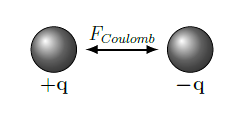
\includegraphics[scale=0.5]{image/chargecharge}	
\caption{Interaction électrostatique entre charges.}
\label{chargecharge}
\end{figure}



\begin{equation}
E_{Coulomb} = \frac{1}{4 \pi \epsilon_{0}} * \frac{q_{1} q_{2}}{r}
\end{equation}

\begin{flushleft}
\begin{tabular}{@{}lrp{10cm}}
avec & $q_{1}$ et $q_{2}$ : & charges respectives des particules 1 et 2, \\
& $r$ : & distance entre les particules. 
\end{tabular}
\end{flushleft}

L'induction est quant à elle due à la déformation de la densité électronique d'un atome ou d'une molécule par l'effet du champ électrique d'une molécule voisine. Ces deux contributions sont très bien définies en physique classique, contrairement à la dispersion et l'échange, qui sont liés à des effets quantiques.
En effet, ce sont les phénomènes de fluctuations quantiques de la distribution des charges qui sont à l'origine du terme de dispersion, et la contribution d'échange est dûe au principe d'exclusion de \textsc{Pauli} qui impose que deux électrons ne peuvent pas posséder le même état quantique au même moment. Dans le cas d'une paire d'atomes en interaction ayant leurs couches électroniques partiellement occupées, cette contribution est positive et engendre une liaison chimique liante forte. À l'inverse, lorsqu'il s'agit de systèmes électroniques à couche fermée, elle devient un terme de répulsion à courte distance responsable du phénomène d'exclusion stérique. Ce phénomène étant inclu dans la loi des \og gaz réels \fg{} de Van der Waals (équation~\ref{GR}) sous la forme du volume d'exclusion $nb$.  


D'une manière plus générale, c'est-à-dire en dépassant le cadre des gaz, les interactions de Van der Waals sont générées par les fluctuations de distributions de charge des atomes et molécules et conduisent aux équations suivantes, où l'énergie est exprimée en Joules :

\begin{align}
E_{Keesom} &= - \frac{1}{r^{6}} \left(\frac{\mu_{1}^{2}\mu_{2}^{2}}{3(4\pi \epsilon_{0} \epsilon)^{2} k_{B}T}\right) \\
E_{Debye} &= - \frac{1}{r^{6}} \left(\frac{\mu_{1}^{2}\alpha_{2}+\mu_{2}^{2}\alpha_{1}}{(4\pi \epsilon_{0} \epsilon)^{2}}\right) \\
E_{London} &= - \frac{1}{r^{6}} \left(\frac{3}{4}\frac{h\nu\alpha_{1}\alpha_{2}}{(4\pi \epsilon_{0})^{2}}\right)
\end{align}

\begin{flushleft}
\begin{tabular}{@{}lrp{10cm}}
avec & $\mu_{1}$ et $\mu_{2}$ : & moments dipolaires respectifs des particules 1 et 2, \\
& $\alpha_{1}$ et $\alpha_{2}$ : & polarisabilités respectives des particules 1 et 2, \\
& $\epsilon_{0}$ : & permittivité diélectrique du vide, \\
& $\epsilon$ : & permittivité diélectrique du milieu, \\
& $k_{B}$ : & constante de \textsc{Boltzmann}, égale à la constante des gaz parfaits $R$ divisée par le nombre d'\textsc{Avogadro} $\mathcal{N}\!a$, \\
& $T$ : & température, \\
& $r$ : & distance entre les particules. \\
\end{tabular}
\end{flushleft}

L'énergie de \textsc{Keesom} (effet d'orientation) représente l'énergie d'interaction entre deux dipôles électrostatiques, c'est-à-dire deux molécules ayant un moment dipolaire\footnote{Le moment dipôlaire d'une molécule résulte d'une répartition hétéroclite de charges électriques, telle que le barycentre des charges positives (noyaux) ne coïncide pas avec celui des charges négatives (électrons), les électrons étant en effet attirés par l'atome le plus électronégatif de la liaison.} $\mu{}$ non nul (figure~\ref{figKeesom}). Il s'agit concrètement de l'attraction mutuelle de deux dipôles permanents qui est d’autant plus forte que les moments dipolaires sont élevés (grande charge et petite taille de la molécule) et que la température est basse.

\begin{figure}[h]
\centering
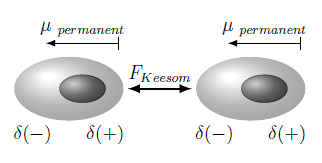
\includegraphics[scale=0.5]{image/Keesom}
\caption{Interaction entre dipôles électrostatiques.}
\label{figKeesom}
\end{figure}

Celle de \textsc{Debye} (effet d'induction) résulte de la déformation du nuage électronique d'une molécule, d'un atome ou d'un ion, par action du champ électrique engendré par le moment dipolaire d'une molécule voisine (figure \ref{figDebye}). Il en résulte ainsi un moment dipolaire induit. Elle est souvent nommé interaction dipôle {permanent-dipôle{ induit et fait intervenir le moment dipolaire $\mu$ et la polarisabilité\footnote{La polarisabilité est la capacité du nuage électronique à se déformer sous l'action d'un champ électrique. Le barycentre des charges négatives (électrons) étant légèrement décalé par rapport à celui des charges positives (noyaux) sous l'effet du champ, un moment électronique induit $\vec{m}_{e}$ apparaît, engendrant la notion de polarisabilité $\alpha$.} $\alpha$ des molécules concernées. Le nominateur $\mu_{1}^{2}\alpha_{2}+\mu_{2}^{2}\alpha_{1}$ décrit l'interaction lorsque les deux molécules sont polaires (cas A) mais s'écrit naturellement $\mu_{1}^{2}\alpha_{2}$ quand la seconde molécule est apolaire (cas B).

% mettre les deux cas dans la figure !
\begin{figure}[h]
\centering
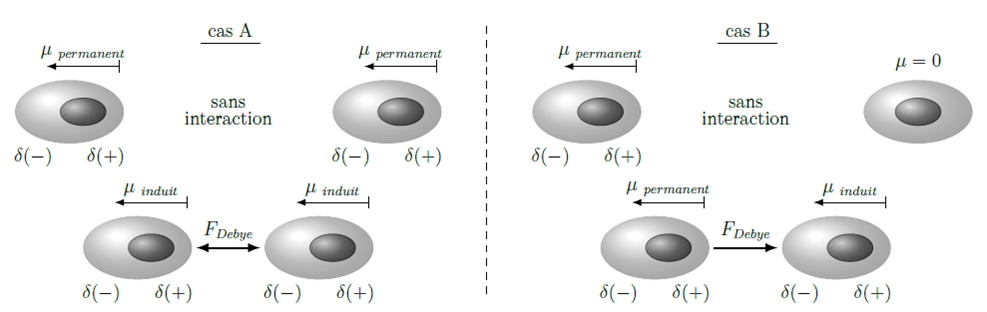
\includegraphics[scale=0.9]{image/Debye}
\caption{Interaction entre une molécule polaire et une seconde polarisable.}
\label{figDebye}
\end{figure}

Finalement, l'énergie de \textsc{London} (effet de dispersion), qui est la plus importante en terme de grandeur, représente l'interaction entre deux dipôles instantanés (figure \ref{figLondon}). Par définition, une molécule apolaire possède un moment dipolaire moyen nul mais la combinaison des mouvements des noyaux et des électrons fait qu'il existe malgré tout un moment dipolaire instantané. Cette interaction est d'autant plus forte que les deux molécules sont facilement polarisables, donc d'autant plus forte que leur taille est importante. Les forces de \textsc{London} étant présentes entre toutes les particules, quelle que soit leur nature, ce sont principalement elles qui permettent la cohésion de la matière dans l'univers.

Notons que les énergies de Van der Waals varient en fonction de l'inverse de la distance à l'ordre 6.

\begin{figure}[h]
\centering
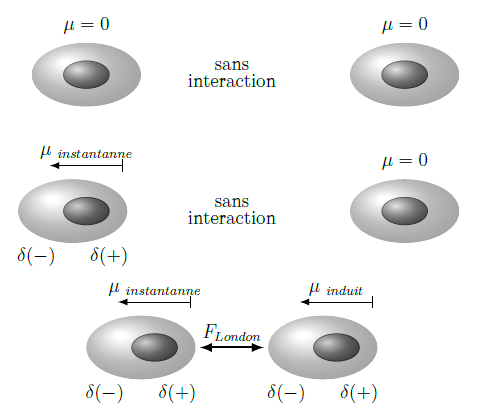
\includegraphics[scale=0.8]{image/London}
\caption{Interaction entre deux dipôles instantanés.}
\label{figLondon}
\end{figure}


Il existe toutefois d'autres types d'interactions électrostatiques que celles décrites par le modèle des forces de VdW. En effet, similaire dans l'esprit à l'énergie de \textsc{Keesom}, l'énergie d'interaction entre un ion et un dipôle permanent est donné par la formule suivante :

\begin{equation}
E_{ion-dipôle} = - \frac{1}{r^{2}} \frac{\mu_{1}q_{2}}{4\pi \epsilon_{0} \epsilon}
\end{equation} 

Il s'agit là encore de l'interaction positive entre une espèce chargée, anion ou cation, et une molécule possédant un moment dipolaire non-nul (\ref{figiondipole}). Ce phénomène est notamment à l'origine de la dissolution des espèces ioniques (ex~:~NaCl) dans un solvant polaire, de l'étape de solvatation qui suit, puis de la bonne dispersion des charges en solution.

\begin{figure}[h]
\centering
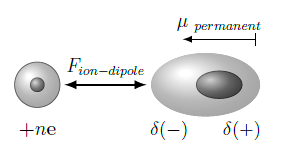
\includegraphics[scale=0.7]{image/Ion-dipole}
\caption{Interaction entre une espèce chargée et une molécule polaire.}
\label{figiondipole}
\end{figure}

De plus, notons aussi la spécificité de la liaison hydrogène qui est une liaison chimique non covalente, de type dipôle-dipôle. Lorsqu'un hétéroatome possédant au moins une paire libre est suffisamment électronégatif (ex : O, N, F), il vient se positionner aux abords d'un hydrogène acide porté par un autre atome fortement électronégatif afin d'en stabiliser la charge partielle $\delta (+)$ ainsi créée.

Bien que de la même famille que les forces de Van der Waals, \textit{i.e.} électrostatique, les liaisons hydrogènes s'en distinguent par une intensité environ dix fois supérieure. Elles restent toutefois une vingtaine de fois plus faibles qu'une liaison covalente. La distance moyenne entre les deux hétéroatomes est de l'ordre de 2,5 \AA .

Dans le cadre de cette thèse, ce sont principalement les interactions entre systèmes conjugués, \textit{i.e.} interactions $\pi-\pi$, qu'il sera nécessaire de traduire. Comme nous pouvons le voir dans le cas simple d'un dimère de benzène représenté en figure \ref{pistackbenz}, l'interaction positive se fait entre les liaisons $\sigma$ et les liaisons $\pi$ alors que les nuages électroniques des liaisons $\pi$ se repoussent naturellement, dû à leurs charges négatives.

Notons que nous retrouvons ce phénomène sous des aspects intramoléculaires, comme par exemple dans le cas de l'hyperconjugaison $\sigma-\pi$ qui vient stabiliser certaines conformations du toluène.

\begin{figure}[h]
\centering
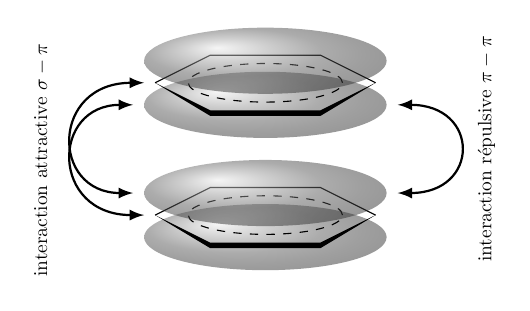
\begin{tikzpicture}[scale=0.7, every node/.style={scale=0.7}]
\shade [shading=ball, ball color=gray, opacity=0.5] (0,0.8) ellipse (2.2cm and 0.6cm) ;
\draw (-2,1.2) --++ (1,0.5) --++ (2,0) --++ (1,-0.5) ;
\fill (-2,1.2) --++ (1,-0.6) --++ (2,0) --++ (1,0.6) --++ (-1,-0.5) --++ (-2,0) -- cycle ;
\draw [dashed] (0,1.2) ellipse (1.4cm and 0.35cm) ;
\shade [shading=ball, ball color=gray, opacity=0.5] (0,1.6) ellipse (2.2cm and 0.6cm) ;
\shade [shading=ball, ball color=gray, opacity=0.5] (0,-1.6) ellipse (2.2cm and 0.6cm) ;
\draw (-2,-1.2) --++ (1,0.5) --++ (2,0) --++ (1,-0.5) ;
\fill (-2,-1.2) --++ (1,-0.6) --++ (2,0) --++ (1,0.6) --++ (-1,-0.5) --++ (-2,0) -- cycle ;
\draw [dashed] (0,-1.2) ellipse (1.4cm and 0.35cm) ;
\shade [shading=ball, ball color=gray, opacity=0.5] (0,-0.8) ellipse (2.2cm and 0.6cm) ;
\draw [latex-latex, thick] (-2.2,-1.2) ..controls +(-1.7,0) and +(-1.5,0).. (-2.4,0.8) node [above, midway, rotate=90, yshift=3mm] {interaction attractive $\sigma - \pi$} ;
\draw [latex-latex, thick] (-2.2,1.2) ..controls +(-1.7,0) and +(-1.5,0).. (-2.4,-0.8) ;
\draw [latex-latex, thick] (2.4,-0.8) ..controls +(1.5,0) and +(1.5,0).. (2.4,0.8) node [below, midway, rotate=90, yshift=-2mm] {interaction répulsive $\pi - \pi$} ;
\end{tikzpicture}
\caption{$\pi$-stacking dans le cas d'un dimère de benzène}
\label{pistackbenz}
\end{figure}

Même si la théorie de la fonctionnelle de la densité connaît un large succès tant elle arrive désormais bien à traduire les phénomènes de liaisons chimiques, les structures géométriques et même la cohésion des solides moléculaires et cristallins, il reste toujours l'obstacle des systèmes chimiques où les forces de Van der Waals sont prédominantes. En effet, les effets de corrélation électronique des forces de dispersion étant purement non-locaux, l'approximation locale ou non-locale qui fait le fondement de la DFT restera problèmatique. Se pose alors la question de savoir comment modéliser ces types d'interaction de façon idiomatique. Nous allons voir que l'élaboration d'une fonctionnelle hybride à longue portée est capable de répondre à cette problèmatique.

\section[LC-DFT-D hybride : $\omega$BXD]{Construction d'une LC-DFT-D hybride : cas de la $\omega$BXD}

Les DFT hybrides avec correction à longue portée basées sur la théorie \textsc{Kohn-Sham} ont naturellement rencontré un grand engouement puisque la précision apportée n'accroît pas le coût calculatoire par rapport aux DFT hybrides.

\subsection{B88}

Comme nous l'avons vu dans le cadre des approximations de la fonctionnelle de la densité, notées DFAs\footnote{\og Density Functional Approximations \fg{} }, la décroissance en exponentielle du potentiel d'échange-corrélation, au lieu d'être en $1/r$, engendre une mauvaise représentation des interactions à longue distance. Cette erreur, nommée erreur d'auto-interaction (SIE, pour \og self-interaction error \fg{}), est liée au fait que ces approximations, basées sur la densité de spin locale (LSDA, pour \og local spin density approximation \fg{}), décrivent mal l'état fondamental qui devrait être, dans le cadre de la DFT pure, strictement sans auto-interaction.     
C'est pourquoi, afin d'introduire un effet non-local de l'échange-corrélation dans le modèle KS-DFT (partie~\ref{Kohn-Sham}), \textsc{Becke} proposa en 1988 d'incorporer dans sa fonctionnelle d'échange B88~\cite{becke1988density} une petite part d'echange exact \textsc{Hartree-Fock}. 

Dans le cadre général des DFAs, l'énergie d'échange-corrélation s'écrit donc :

\begin{equation}
E_{xc} = c_{x}E_{x}^{HF} + E_{xc}^{DFA}
\label{xcB88}
\end{equation}

\noindent où $c_{x}$ prend généralement des valeurs comprises entre 0,2 et 0,25~\cite{becke1993density} pour les données thermodynamiques et entre 0,4 et 0,6~\cite{boese2004development} pour les études cinétiques.

Basée sur ce modèle, la désormais bien connue DFT hybride B3LYP \cite{becke1993density} (équation~\ref{B3LYP}) donne des résultats comparables à ceux obtenus à partir de la théorie perturbative \textsc{M\o ller-Plesset} à l'ordre 2 \cite{moller1934note}, noté MP2, souvent utilisée comme référence, dans le cadre de systèmes fortement liés. Depuis, de nombreuses recherches ont porté sur l'amélioration constante de ce potentiel d'échange-corrélation $E_{xc}[\rho]$.

\subsection{B97}

Une avancée significative a de nouveau été faite par \textsc{Becke} en 1997 dans le domaine des KS-DFT. Par une méthode similaire à la combinaison linéaire d'orbitales atomiques, notée LCAO\footnote{\og Linear Combination of Atomic Orbitals \fg{}.}, il a proposé un modèle mathématique basé sur l'approximation de densité de spin local (LSDA), sa première dérivée et une petite fraction d'échange HF pour décrire le potentiel d'échange-corrélation $E_{xc}[\rho]$. Une optimisation systématique des coefficients linéaires à partir d'un jeu classique de données expérimentales a conduit à l'apparition de la méthode B97~\cite{becke1997density}. La base de données contient notamment des valeurs relatives à l'interaction entre systèmes conjugués.

Cette méthodologie a été reprise par F. A. \textsc{Hamprecht} et al, P. J. \textsc{Wilson} et al et T. W. \textsc{Keal} et al pour respectivement conduire à la B97-1 \cite{hamprecht1998development} (1998), la B97-2 \cite{wilson2001hybrid} (2001) et la B97-3 \cite{keal2005semiempirical} (2005). Il s'agissait alors de réoptimisations des coefficients linéaires par rapport à d'autres bases de données expérimentales plus complètes.

Mais cette reparamétrisation empirique du terme d'échange-corrélation ne résout pas le problème de sa non-décroissance en $1/r$. La prise en compte totale du terme d'échange HF $E_{x}^{HF}$ ($c_{x}$=1 dans l'équation~\ref{xcB88}) pourait résoudre ce problème mais cela serait incompatible avec le terme de corrélation DFA $E_{c}^{DFA}$. En effet, il existerait alors une mauvaise compensation des erreurs respectives.

\subsection{$\omega$B97}

L'idée de séparer le traitement des interactions courtes (SR, pour \og short range \fg{}) et longues portées (LR, pour \og long range \fg{}) s'est alors présentée comme le choix le plus évident, aussi bien au niveau de la compréhension des phénomènes que mathématiquement parlant. Nous pouvons ainsi traiter séparément à l'aide d'une fonction erreur $(erf)$ les interactions à courtes distances par une fonctionnelle de la densité et celles longue distance par une fonction d'onde. Ce principe conduit naturellement à l'élaboration d'une fonctionnelle hybride à séparation de portée. L'introduction de la fonction erreur, avec un paramètre libre, permet de contrôler le rayon d'action des interactions de courte-portée.

La première proposition faite par \textsc{Iikura} et al \cite{iikura2001long} a été de traiter la partie d'échange LR par la théorie HF alors que la partie SR est approximée par une DFA; le terme de corrélation est quant à lui le même que celui de \textsc{Coulomb}, quelle que soit la distance :

\begin{equation}
E_{xc}^{LC-DFA} = E_{x}^{LR-HF} + E_{x}^{SR-DFA} + E_{c}^{DFA}
\end{equation}

Ce schéma de séparation de portée a l'avantage de conduire à des temps de calcul très proches des DFT hybrides, mais il reste à développer une fonctionnelle d'échange SR précise et une fonctionnelle de corrélation qui soit entièrement compatible entre elles.

Le type d'opérateur de coupure le plus utilisé dans le cadre des LC-DFT hybrides est la fonction d'erreur standard $(erf)$ :

\begin{equation}
\frac{1}{r} = \frac{erf(\omega r_{12})}{r_{12}} + \frac{erfc(\omega r_{12})}{r_{12}}
\label{erf}
\end{equation}

\begin{flushleft}
\begin{tabular}{@{}lrp{10cm}}
avec & $\frac{erf(\omega r_{12})}{r_{12}}$ : & interaction de courte portée, \\
& $\frac{erfc(\omega r_{12})}{r_{12}}$ : & interaction complémentaire, \\
& $r_{12}$ : & distance entre les particules 1 et 2, \\
& $\omega$ : & paramètre contrôlant la séparation.
\end{tabular}
\end{flushleft}

Notons que l'introduction du paramètre $\omega$, qui s'exprime comme l'inverse d'une distance, permet de donner un sens physique à cette valeur, en cela qu'il est étroitement lié à une longueur caractéristique de la séparation.
Naturellement, il existe différents types de fonctions erreur $(erf)$ afin de faciliter son intégration mathématique dans les codes de calculs. Dans le cas de la $\omega$B97 \cite{chai2008long} et, par conséquent, des fonctionnelles $\omega$B97X et $\omega$B97X-D, c'est la fonction $erf/erfc$ qui a été choisie par Jeng-Da \textsc{Chai} et Martin \textsc{Head-Gordon} dans leurs travaux. \\

Le choix des auteurs s'est porté sur un terme d'échange exact HF longue portée $E_{x}^{LR-HF}$, calculé à partir des spin-orbitales occupées $\phi_{i \sigma}(r)$, et une forme analytique du terme d'échange $E_{x}^{SR-DFA}$ obtenue par l'intégration du carré de la matrice densité LSDA :

\begin{align}
E_{x}^{LR-HF} &= -\frac{1}{2} \sum_{\sigma} \sum_{ij}^{occ.} \iint \phi_{i \sigma}^{*}(r_{1}) \phi_{j \sigma}^{*}(r_{1}) \frac{erf(\omega r_{12})}{r_{12}} \phi_{i \sigma}(r_{2}) \phi_{j \sigma}(r_{2}).dr_{1}.dr_{2}, \\
E_{x}^{SR-LSDA} &= \sum_{\sigma} \int \underbrace{-\frac{3}{2}\left(\frac{3}{4\pi}\right)^{1/3}\rho_{\sigma}^{4/3} (r) F(a_{\sigma})}_{e_{x \sigma}^{SR-LSDA} (\rho_{\sigma}) .dr}.
\end{align}

\noindent où :
\begin{align}
k_{F \sigma}&=(6\pi^{2}\rho_{sigma}(r))^{1/3},\nonumber\\
F(a_{\sigma})&=1-\frac{8}{3}a_{\sigma}\left[\sqrt{\pi}\: erf\left(\frac{1}{2a_{\sigma}}\right)-3a_{\sigma}+4a_{\sigma}^{3}+(2a_{\sigma}-4a_{\sigma}^{3}) \: exp\left(-\frac{1}{4a_{\sigma}^{2}}\right)\right],\nonumber\\
a_{\sigma}&=\frac{\omega}{2k_{F\sigma}}.\nonumber
\end{align}

\begin{flushleft}
\begin{tabular}{@{}lrp{10cm}}
avec & $k_{F\sigma}$ : & vecteur d'onde local de Fermi,\\
& $F(a_{\sigma})$ : & fonction d'atténuation,\\
& $a_{\sigma}$ : & paramètre de contrôle (sans unité) de la fonction d'atténuation $F(a_{\sigma})$.
\end{tabular}
\end{flushleft}

En retenant une fonctionnelle de corrélation basée elle aussi sur la LSDA $E_{c}^{LSDA}$, la plus simple des DFT hybrides à correction de longue portée (RSHX-LDA) s'écrit~:

\begin{equation}
E_{xc}^{RSHXLDA} = E_{x}^{LR-HF} + E_{x}^{SR-LSDA} + E_{c}^{LSDA}
\end{equation}

La fonctionnelle $\omega$B97\cite{chai2008long} s'écrit alors :

\begin{equation}
E_{xc}^{\omega B97} = E_{x}^{LR-HF} + E_{x}^{SR-B97} + E_{c}^{B97}
\end{equation}

Il est à noter que celle-ci ne possède pas d'échange \textsc{Hartree-Fock} à courte portée (SR), comme la plupart des fonctionnelles hybrides à correction de portée.

Malgré plusieurs études visant à optimiser la valeur du paramètre $\omega$, la précision calculatoire reste insuffisante en terme de thermochimie. En effet, nous l'avons déjà vu, une valeur trop grande pour $\omega$ tendrait vers une incompatibilité entre le terme d'échange non-local $E_{x}^{LR-HF}$ et le terme local de corrélation $E_{c}^{LSDA}$. De plus, nous pouvons aisément comprendre, d'après l'équation~\ref{erf}, que plus $\omega$ est petit, plus la contribution du terme d'échange SR $E_{x}^{SR-LSDA}$ sera importante. L'utilisation d'une trop faible valeur  reviendrait alors à traiter le problème dans un cadre très proche de la LDA classique qui, comme nous l'avons vu dans la partie~\ref{lda}, est incapable de traduire correctement le terme d'échange à courte portée.

\subsection{$\omega$B97X}

Afin d'y remédier, une partie d'échange SR HF $E_{x}^{SR-HF}$, est ajoutée à $E_{x}^{SR-LSDA}$ dans une proportion d'environ 16\%,  de la même manière que \textsc{Becke} dans la fonctionnelle B88. Ceci à l'avantage de ne pas perturber la partie LR qui est dorénavant correcte. Ainsi, la nouvelle fonctionnelle comporte désormais un paramètre $c_{x}$ contrôlant la proportion d'échange exact HF à courte distance, comme nous pouvons le voir dans son expression :

\begin{equation}
E_{xc}^{LC-DFA} = E_{x}^{LR-HF} + c_{x}E_{x}^{SR-HF} + E_{x}^{SR-DFA} + E_{c}^{DFA}
\end{equation}

\noindent où :

\begin{equation}
E_{x}^{SR-HF} = -\frac{1}{2} \sum_{\sigma} \sum_{ij}^{occ.} \iint \phi_{i \sigma}^{*}(r_{1}) \phi_{j \sigma}^{*}(r_{1}) \frac{erfc(\omega r_{12})}{r_{12}} \phi_{i \sigma}(r_{2}) \phi_{j \sigma}(r_{2}).dr_{1}.dr_{2}, \\
\end{equation}

C'est ainsi que la fonctionnelle $\omega$B7X\cite{chai2008long} se décompose de la façon suivante~:

\begin{equation}
E_{xc}^{\omega B97X} = E_{x}^{LR-HF} + c_{x}E_{x}^{SR-HF} + E_{x}^{SR-B97} + E_{c}^{B97}
\end{equation}

La valeur de $\omega$, comme les valeurs des coefficients de développements linéaires et de développements à l'ordre $m$ des fonctionnelles $\omega$B97 et $\omega$B97X ont été déterminées par la méthode des moindres carrés appliquée à une base de données composées de 412 valeurs précises, expérimentales et théoriques.

Malgré toutes ces optimisations conduisant à une bien meilleure représentation des systèmes en interaction, ces fonctionnelles connaissent encore des lacunes quant à la traduction des interactions de dispersion entre atomes, ie les forces de \textsc{London}. Comme nous allons le voir dans le cas de la fonctionnelle $\omega$B97X-D, ceci peut être corrigé par une prise en compte empirique des effets de dispersion.

\subsection{$\omega$B97X-D}

Cette dernière correction pourrait naturellement passer par le calcul idiomatique de l'énergie de dispersion entre chaque atome, mais cela occasionnerait alors un coût calculatoire prohibitif. C'est pourquoi Jeng-Da \textsc{Chai} et Martin \textsc{Head-Gordon} ont fait le choix d'appliquer cette correction de façon empirique par l'ajout d'un terme $E_{disp}$ à la fonctionnelle KS-DFT, ici la $\omega$B97X. L'expression de l'énergie de la fonctionnelle $\omega$B97X-D \cite{chai2008long} ainsi créée devient alors :

\begin{equation}
E_{DFT-D}=E_{\omega B97X}+E_{disp}
\end{equation}

L'énergie de dispersion $E_{disp}$ est définie par rapport à une fonction d'amortissement $f_{damp}$ :

\begin{equation}
E_{disp}=-\sum_{i-1}^{N_{at}-1} \sum_{j-i+1}^{N_{at}} \frac{C_{6}^{ij}}{R_{ij}^{6}}f_{damp} (R_{ij})
\end{equation}

\noindent où :
\begin{equation}
f_{damp} (R_{ij})=\frac{1}{1+a(\frac{R_{ij}}{R_{r}})^{-12}}
\end{equation}

Une nouvelle fois, la partie empirique a été paramétrée par rapport à la même base de données que pour les fonctionnelles $\omega$B97 et $\omega$BX97.


\newpage

\section*{Conclusion}
\markright{CONCLUSION}{}

En résumé, l'apport de la fonction erreur $(erf)$ permet de mieux gérer les contributions d'échange-corrélation selon la distance d'interaction. Les DFT hybrides $\omega$B97 et $\omega$B97X prennent ainsi en compte la totalité de l'échange exact à longue distance et utilisent la méthode des gradients généralisés à faible distance, alors que la corrélation électronique reste basée sur celle initialement développée par \textsc{Becke} dans la fonctionnelle B97. Ceci a pour effet de supprimer le problème d'auto-interaction de la fonctionnelle d'échange à longue distance.

Les travaux de Jeng-Da \textsc{Chai} et Martin \textsc{Head-Gordon} ont finalement conduit à la fonctionnelle $\omega$B9X-D, de type LC-DFT-D hybride, où la totalité de l'échange exact HF est pris en compte à longue distance, en même temps qu'une petite partie -- environ 22 \% -- de l'échange exact HF est introduite à courte distance pour compléter une fonctionnelle d'échange B97 modifiée ; une correction empirique de la dispersion est finalement appliquée.

Comme toutes les fonctionnelles LC-DFT, le problème de l'auto-interaction est corrigé à longue distance mais reste quelque peu présent à courte distance. Les effets de corrélation à longue distance sont quant à eux purement et simplement traités par la correction empirique de dispersion.

Cette fonctionnelle est, d'après les tests des auteurs, définitivement plus adaptée à l'étude de systèmes chimiques où les interactions non-covalentes sont importantes.






